\section{Интерференция}

\textbf{12.03.}

\begin{definition}{Интерференция}{interference}
	\textbf{Интерференция} --- перераспределение энергии в пространстве при наложении волн. При наложении пучков света, результирующая интенсивность не равна сумме:
	\begin{equation*}
		I \neq I_1 + I_2
	\end{equation*}
\end{definition}

Запишем уравнения волн:
\begin{align*}
	\vb{E}_1 &= \vb{e}_1 a \cdot e^{i \varphi_1}, \quad \varphi = \qty(\omega t - \vb{k}\vb{r} + \varphi_0) \\
	\vb{E}_2 &= \vb{e}_2 b \cdot e^{i \varphi_2}, \quad \vb{E} = \vb{E}_1 + \vb{E}_2
\end{align*}

Интенсивность $I \sim \abs{\vb{E}}^2$, где $\abs{\vb{E}}^2 = \vb{E}\vb{E}^* = (\vb{E}_1 + \vb{E}_2)(\vb{E}_1^* + \vb{E}_2^*) = \vb{E}_1\vb{E}_1^* + \vb{E}_2\vb{E}_2^* + \vb{E}_1\vb{E}_2^* + \vb{E}_2\vb{E}_1^*$.

\begin{multline*}
	I = a^2 + b^2 + (\vb{e}_1, \vb{e}_2) ab \cdot \exp(i(\varphi_1 - \varphi_2)) + (\vb{e}_1, \vb{e}_2) ab \cdot \exp(-i(\varphi_1 - \varphi_2)) = \\
	= I_1 + I_2 + (\vb{e}_1, \vb{e}_2) ab \qty[e^{i(\varphi_1 - \varphi_2)} + e^{-i(\varphi_1 - \varphi_2)}]
\end{multline*}

\begin{nb}
	\begin{equation}
		I = I_1 + I_2 + 2(\vb{e}_1, \vb{e}_2)\sqrt{I_1 I_2} \cos(\varphi_1 - \varphi_2)
	\end{equation}
	--- общая интенсивность результирующей волны.
\end{nb}

\begin{itemize}
	\item Ортогонально-поляризованные волны \textbf{не} интерферируют: 
	$\vb{e}_1 \perp \vb{e}_2 \implies (\vb{e}_1, \vb{e}_2) = 0 \implies I = I_1 + I_2$.
	
	\item Если поляризация параллельная: $\vb{e}_1 \parallel \vb{e}_2$.
	\begin{equation*}
		\begin{cases}
			I_{\text{max}} = I_1 + I_2 + 2\sqrt{I_1 I_2} = \qty(\sqrt{I_1} + \sqrt{I_2})^2 \\
			\qquad \cos\Delta\varphi = 1, \quad \Delta\varphi = 2\pi m, \quad m = 0, 1, 2, \dots \\
			I_{\text{min}} = I_1 + I_2 - 2\sqrt{I_1 I_2} = \qty(\sqrt{I_1} - \sqrt{I_2})^2 \\
			\qquad \cos\Delta\varphi = -1, \quad \Delta\varphi = \pi(2m+1), \quad m = 0, 1, 2, \dots
		\end{cases}
	\end{equation*}
\end{itemize}

\begin{figure}[H]
	\centering
	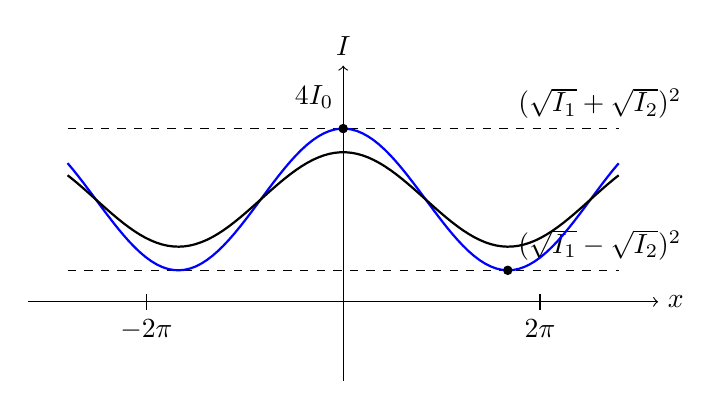
\begin{tikzpicture}
		% Axes
		\draw[->] (-4, 0) -- (4, 0) node[right] {$x$};
		\draw[->] (0, -1) -- (0, 3) node[above] {$I$};
		
		% Ticks
		\draw (-2.5, 0.1) -- (-2.5, -0.1) node[below] {$-2\pi$};
		\draw (2.5, 0.1) -- (2.5, -0.1) node[below] {$2\pi$};
		
		% I_max and I_min lines
		\draw[dashed] (-3.5, 2.2) -- (3.5, 2.2) node[above right, pos=0.8] {$(\sqrt{I_1} + \sqrt{I_2})^2$};
		\draw[dashed] (-3.5, 0.4) -- (3.5, 0.4) node[above right, pos=0.8] {$(\sqrt{I_1} - \sqrt{I_2})^2$};
		
		% Interference curve (I_1 = I_2 case)
		\draw[blue, thick, domain=-3.5:3.5, samples=100] plot (\x, {1.3 + 0.9*cos(deg(1.5*\x))});
		
		% I_1 != I_2 case
		\draw[black, thick, domain=-3.5:3.5, samples=100] plot (\x, {1.3 + 0.6*cos(deg(1.5*\x))});
		
		% Annotations
		\node[left] at (0, 2.6) {$4I_0$};
		\filldraw (0, 2.2) circle (1.5pt);
		\filldraw (2.09, 0.4) circle (1.5pt);
	\end{tikzpicture}
\end{figure}

Если $I_1 = I_2 \equiv I_0$:
\begin{align*}
	I &= 2I_0(1 + \cos\Delta\varphi) = 4I_0 \cos^2\frac{\Delta\varphi}{2} \\
	I_{\text{max}} &= 4I_0 \\
	I_{\text{min}} &= 0
\end{align*}

\begin{definition}{Видность}{visibility}
	Количественная характеристика, отражающая степень контрастности интерференционной картинки:
	\begin{equation}
		V = \frac{I_{\text{max}} - I_{\text{min}}}{I_{\text{max}} + I_{\text{min}}}
	\end{equation}
	Если $V=0 \implies I_{\text{max}} = I_{\text{min}}$. Если $V=1 \implies I_{\text{min}} = 0$. ($0 \le V \le 1$).
\end{definition}

\begin{nb}
	\textbf{Когерентность} --- * важное условие интерференции! \\
	$\hookrightarrow$ когда $\Delta \varphi = \text{const}$ $\hookrightarrow$ необходимое условие устойчивости интерференционной картинки.
\end{nb}

Пусть $\varphi = \omega t - \vb{k}\vb{r} + \varphi_0$.
\begin{equation*}
	\Delta\varphi = \qty[(\omega_1 - \omega_2)t - (\vb{k}_1\vb{r}_1 - \vb{k}_2\vb{r}_2) + \varphi_{01} - \varphi_{02}]
\end{equation*}
Отсюда следует $\omega_1 = \omega_2$. Волны разных частот \textbf{не} интерферируют.
\begin{equation*}
	\varphi_{01} = \varphi_{02}, \quad \omega_1 = \omega_2, \quad \Delta\varphi = \varphi_1 - \varphi_2 = - \vb{k}_1\vb{r}_1 + \vb{k}_2\vb{r}_2 = \text{const}
\end{equation*}

\begin{equation*}
	\Delta\varphi = \frac{2\pi}{\lambda} n_1 r_1 - \frac{2\pi}{\lambda} n_2 r_2 = \frac{2\pi}{\lambda} \underbrace{(n_1 r_1 - n_2 r_2)}_{\text{оптическая разность хода } \Delta} = \frac{2\pi}{\lambda} \Delta \qquad \text{* } k = \frac{\omega}{v}, \; n = \frac{c}{v}
\end{equation*}
$\lambda$ --- длина волны в вакууме.

* Если среды неоднородны: $\Delta = \int n_1(l) \dd{l} - \int n_2(l) \dd{l}$.
\begin{equation*}
	\begin{cases}
		\text{условие max:} \quad \Delta\varphi = 2\pi m \implies \frac{2\pi}{\lambda}\Delta = 2\pi m \implies \Delta = \lambda m \\
		\text{условие min:} \quad \Delta\varphi = \pi(2m+1) \implies \frac{2\pi}{\lambda}\Delta = \pi(2m+1) \implies \Delta = \lambda\qty(m + \frac{1}{2})
	\end{cases}
\end{equation*}

\begin{figure}[H]
	\centering
	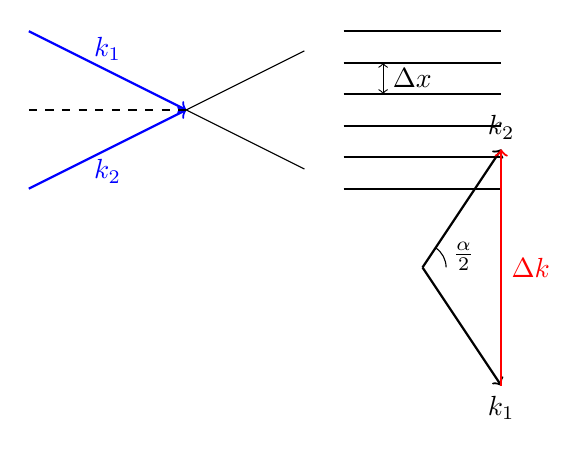
\begin{tikzpicture}
		% Two crossing plane waves
		\draw[->, thick, blue] (-2, 1) -- (0, 0) node[pos=0.5, above] {$\vb{k}_1$};
		\draw[->, thick, blue] (-2, -1) -- (0, 0) node[pos=0.5, below] {$\vb{k}_2$};
		\draw[dashed] (-2,0) -- (0,0);
		
		\draw (0,0) -- (1.5, 0.75);
		\draw (0,0) -- (1.5, -0.75);
		
		% Fringes
		\foreach \y in {-1, -0.6, -0.2, 0.2, 0.6, 1} {
			\draw[thick] (2, \y) -- (4, \y);
		}
		\draw[<->] (2.5, 0.2) -- (2.5, 0.6) node[midway, right] {$\Delta x$};
		
		% Vector triangle
		\begin{scope}[shift={(3, -2)}]
			\draw[->, thick] (0,0) -- (1, 1.5) node[above] {$\vb{k}_2$};
			\draw[->, thick] (0,0) -- (1, -1.5) node[below] {$\vb{k}_1$};
			\draw[->, thick, red] (1, -1.5) -- (1, 1.5) node[midway, right] {$\Delta \vb{k}$};
			\draw (0.3, 0) arc (0:56:0.3) node[midway, right] {$\frac{\alpha}{2}$};
		\end{scope}
	\end{tikzpicture}
\end{figure}

Пусть $k_1 = k_2$, $(\widehat{\vb{k}_1, \vb{k}_2}) = \alpha$. $\Delta x$ --- ширина полосы интерференции.
\begin{align*}
	\Delta\varphi &= \Delta k \Delta x \\
	\Delta k &= 2k \sin\frac{\alpha}{2} = 2 \cdot \frac{2\pi}{\lambda} \sin\frac{\alpha}{2} \\
	\Delta x \cdot 2 \cdot \frac{2\pi}{\lambda} \sin\frac{\alpha}{2} &= 2\pi \implies \Delta x = \frac{\lambda}{2 \sin(\alpha/2)} \quad \text{Если } \alpha \to 0 \implies \Delta x \sim \frac{\lambda}{\alpha}
\end{align*}

\begin{nb}
	Порядок интерференции: $m = \frac{x}{\Delta x}$ \\
	Интенсивность: $I(x) = 4I_0 \cos^2\qty(\frac{\pi x}{\Delta x})$ --- периодическое поле.
\end{nb}

\subsection{Способы наблюдения интерференции}

\subsubsection{(1) Интерференционные опыты с делением волнового фронта}
Волну, излуч. одним источником света, разделяют тем или иным способом на две или раскладывают друг на друга.

\textbf{Опыт Юнга.}

\begin{figure}[H]
	\centering
	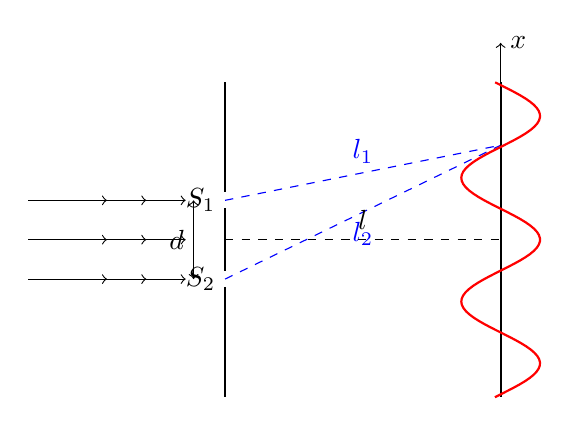
\begin{tikzpicture}
		% Light source
		\foreach \x in {-1, -0.5, 0} {
			\draw[->] (\x, 0.5) -- (\x + 1, 0.5);
			\draw[->] (\x, -0.5) -- (\x + 1, -0.5);
			\draw[->] (\x, 0) -- (\x + 1, 0);
		}
		
		% First screen with 2 slits
		\draw[thick] (1.5, 2) -- (1.5, 0.6);
		\draw[thick] (1.5, 0.4) -- (1.5, -0.4);
		\draw[thick] (1.5, -0.6) -- (1.5, -2);
		
		\node[left] at (1.5, 0.5) {$S_1$};
		\node[left] at (1.5, -0.5) {$S_2$};
		
		% Rays to screen
		\draw[blue, dashed] (1.5, 0.5) -- (5, 1.2) node[midway, above] {$l_1$};
		\draw[blue, dashed] (1.5, -0.5) -- (5, 1.2) node[midway, below] {$l_2$};
		\draw[dashed] (1.5, 0) -- (5, 0) node[midway, above] {$l$};
		
		% Screen
		\draw[thick] (5, 2) -- (5, -2);
		\draw[->] (5, 0) -- (5, 2.5) node[right] {$x$};
		
		% Distance annotations
		\draw[<->] (1.1, 0.5) -- (1.1, -0.5) node[midway, left] {$d$};
		
		% Interference pattern
		\draw[red, thick, domain=-2:2, samples=100] plot ({5 + 0.5*cos(deg(4*\x))}, \x);
	\end{tikzpicture}
\end{figure}

В вакууме:
\begin{align*}
	\Delta &= l_2 - l_1 = \sqrt{\qty(x + \frac{d}{2})^2 + l^2} - \sqrt{\qty(x - \frac{d}{2})^2 + l^2} = l \sqrt{1 + \frac{(x+d/2)^2}{l^2}} - l \sqrt{1 + \frac{(x-d/2)^2}{l^2}} \approx \\
	&\approx l \qty[1 + \frac{1}{2} \frac{(x+d/2)^2}{l^2} - 1 - \frac{1}{2}\frac{(x-d/2)^2}{l^2}] = \\
	&= \frac{l}{2l^2} \qty[ \qty(x^2 + dx + \frac{d^2}{4}) - \qty(x^2 - dx + \frac{d^2}{4}) ] = \frac{dx}{l}
\end{align*}
где использовалось разложение $(1+x)^\alpha \approx 1 + \alpha x$ при $x \ll 1$.

\begin{equation}
	\Delta = \frac{dx}{l} - \text{угловой размер щелей} \qquad \Delta x = \frac{\lambda}{\psi}
\end{equation}

Условие максимума $\Delta = m\lambda$:
\begin{equation}
	\frac{dx}{l} = m\lambda \implies x_m = \frac{m\lambda l}{d} \implies \Delta x = \frac{\lambda l}{d} \text{ --- ширина интерф. полосы для опыта Юнга}
\end{equation}
Обычно $d \sim 10^{-1} - 10^{-2}$ мм.

\textbf{Бипризма Френеля} (аналог опыта Юнга).

\begin{figure}[H]
	\centering
	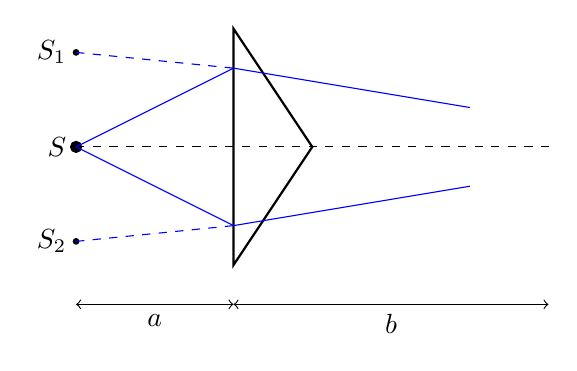
\begin{tikzpicture}
		% Source
		\filldraw (0,0) circle (2pt) node[left] {$S$};
		
		% Biprism
		\draw[thick] (2, 1.5) -- (2, -1.5) -- (3, 0) -- cycle;
		\draw[dashed] (0,0) -- (6,0);
		
		% Virtual sources
		\filldraw (0, 1.2) circle (1pt) node[left] {$S_1$};
		\filldraw (0, -1.2) circle (1pt) node[left] {$S_2$};
		
		% Rays
		\draw[blue] (0,0) -- (2, 1) -- (5, 0.5);
		\draw[blue] (0,0) -- (2, -1) -- (5, -0.5);
		\draw[dashed, blue] (0, 1.2) -- (2, 1);
		\draw[dashed, blue] (0, -1.2) -- (2, -1);
		
		\draw[<->] (0, -2) -- (2, -2) node[midway, below] {$a$};
		\draw[<->] (2, -2) -- (6, -2) node[midway, below] {$b$};
	\end{tikzpicture}
\end{figure}

\begin{align*}
	\Delta &= \frac{dx}{l} = \frac{2 x a (\theta-1)}{a+b} \quad \text{-- разность хода} \\
	\frac{d}{2} &= a \tg\varphi \approx a\varphi = a\theta(n-1) \implies d = 2a\theta(n-1) \\
	\varphi &= \theta(n-1) \text{ --- отклонение лучей призмы} \qquad \text{*углы у нас малые} \\
	\Delta x &= \frac{(a+b)\lambda}{2a\theta(n-1)}
\end{align*}

\textbf{Билинза Бийе.}
\begin{figure}[H]
	\centering
	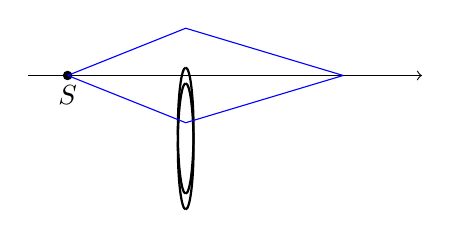
\begin{tikzpicture}
		\draw[->] (-2,0) -- (3,0);
		\filldraw (-1.5, 0) circle (1.5pt) node[below] {$S$};
		
		% Split lens
		\draw[thick] (0, 0.1) arc (90:270:0.1 and 0.8);
		\draw[thick] (0, 0.1) arc (90:-90:0.1 and 0.8);
		
		\draw[thick] (0, -0.1) arc (90:270:0.1 and 0.8);
		\draw[thick] (0, -0.1) arc (90:-90:0.1 and 0.8);
		
		% Rays
		\draw[blue] (-1.5, 0) -- (0, 0.6) -- (2, 0);
		\draw[blue] (-1.5, 0) -- (0, -0.6) -- (2, 0);
	\end{tikzpicture}
\end{figure}

\textbf{Зеркало Ллойда.}
\begin{figure}[H]
	\centering
	\begin{tikzpicture}
		\draw[thick] (0,0) -- (2,0);
		\filldraw (-1, 1) circle (1.5pt) node[left] {$S$};
		\filldraw (-1, -1) circle (1pt) node[left] {$S^*$};
		\draw[dashed] (-1, 1) -- (-1, -1);
		
		\draw[blue] (-1, 1) -- (1, 0) -- (3, 1);
		\draw[blue, dashed] (-1, -1) -- (1, 0);
	\end{tikzpicture}
\end{figure}

\subsubsection{(2) Интерференционные опыты с делением амплитуды}
Используется тот же участок волнового фронта. Деление одной волны на две - за счет частичного отражения/пропускания на границе двух прозрачных сред.

\textbf{Интерференция на тонкой пленке}
\begin{figure}[H]
	\centering
	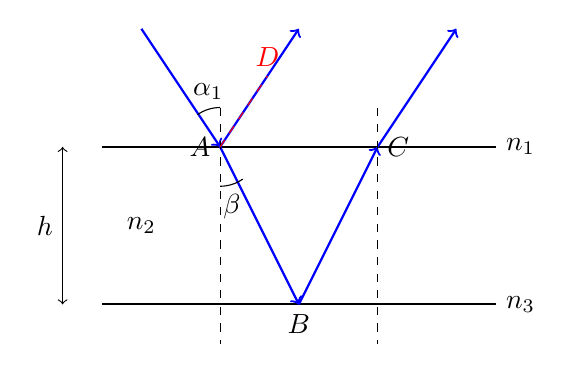
\begin{tikzpicture}
		% Film
		\draw[thick] (0, 2) -- (5, 2) node[right] {$n_1$};
		\draw[thick] (0, 0) -- (5, 0) node[right] {$n_3$};
		\node at (0.5, 1) {$n_2$};
		
		\draw[<->] (-0.5, 0) -- (-0.5, 2) node[midway, left] {$h$};
		
		% Ray
		\draw[blue, thick, ->] (0.5, 3.5) -- (1.5, 2);
		\draw[blue, thick, ->] (1.5, 2) -- (2.5, 0);
		\draw[blue, thick, ->] (2.5, 0) -- (3.5, 2);
		\draw[blue, thick, ->] (3.5, 2) -- (4.5, 3.5);
		\draw[blue, thick, ->] (1.5, 2) -- (2.5, 3.5);
		
		% Normals
		\draw[dashed] (1.5, 2.5) -- (1.5, -0.5);
		\draw[dashed] (3.5, 2.5) -- (3.5, -0.5);
		
		% Points
		\node[left] at (1.5, 2) {$A$};
		\node[below] at (2.5, 0) {$B$};
		\node[right] at (3.5, 2) {$C$};
		
		% Perpendicular wavefront
		\draw[dashed, red] (1.5, 2) -- (2.1, 2.9) node[above] {$D$};
		
		% Angles
		\draw (1.5, 2.5) arc (90:125:0.5) node[midway, above] {$\alpha_1$};
		\draw (1.5, 1.5) arc (270:305:0.5) node[midway, below] {$\beta$};
	\end{tikzpicture}
\end{figure}

\begin{align*}
	\Delta &= n_2 l_2 - n_1 l_1 \qquad l_2 = AB + BC \\
	l_1 &= AD \\
	l_2 &= \frac{2h}{\cos\beta} \\
	l_1 &= 2h \tg\beta \cdot \sin\alpha \\
	\Delta &= \frac{2h n_2}{\cos\beta} - 2hn_1 \tg\beta \cdot \sin\alpha = \frac{2hn_2}{\cos\beta} \qty[1 - \frac{n_1}{n_2} \sin\alpha \sin\beta] = \frac{2hn_2}{\cos\beta} \qty(1 - \sin^2\beta) = \\
	&= 2h n_2 \cos\beta = 2h n_2 \sqrt{1 - \sin^2\beta} = 2h n_2 \sqrt{1 - \qty(\frac{n_1}{n_2})^2 \sin^2\alpha} = 2h \sqrt{n_2^2 - n_1^2 \sin^2\alpha} \pm \frac{\lambda}{2}
\end{align*}
$\pm \frac{\lambda}{2}$ возникает при отражении (потеря полуволны). 
\begin{equation*}
	\Delta = 
	\begin{cases}
		\Delta \pm \frac{\lambda}{2} \quad &n_1 < n_2 > n_3 \\
		&n_1 > n_2 < n_3 \\
		\Delta \quad &n_1 < n_2 < n_3 \\
		&n_1 > n_2 > n_3
	\end{cases}
\end{equation*}

\begin{itemize}
	\item Условие max: $\Delta = m\lambda \implies m\lambda = 2h\sqrt{n_2^2 - n_1^2 \sin^2\alpha} \pm \frac{\lambda}{2}$.
	\item Условие min: $\qty(m + \frac{1}{2})\lambda = 2h\sqrt{n_2^2 - n_1^2 \sin^2\alpha} \pm \frac{\lambda}{2}$.
\end{itemize}

\textbf{Локализация на поверхности:}
Пленка переменной толщины:
\begin{equation*}
	2hn \pm \frac{\lambda}{2} = m\lambda
\end{equation*}

\textbf{Кольца Ньютона}
\begin{figure}[H]
	\centering
	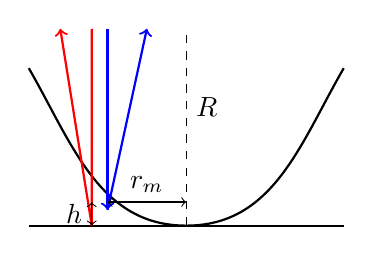
\begin{tikzpicture}
		% Flat plate
		\draw[thick] (-2, 0) -- (2, 0);
		
		% Lens
		\draw[thick] (-2, 2) to[out=-60, in=180] (0, 0) to[out=0, in=240] (2, 2);
		\draw[dashed] (0,0) -- (0, 2.5);
		
		% Rays
		\draw[blue, thick, ->] (-1, 2.5) -- (-1, 0.2);
		\draw[blue, thick, ->] (-1, 0.2) -- (-0.5, 2.5);
		\draw[red, thick, ->] (-1.2, 2.5) -- (-1.2, 0) -- (-1.6, 2.5);
		
		\draw[<->] (0, 0.3) -- (-1, 0.3) node[midway, above] {$r_m$};
		\draw[<->] (-1.2, 0) -- (-1.2, 0.3) node[midway, left] {$h$};
		
		\node[right] at (0, 1.5) {$R$};
	\end{tikzpicture}
\end{figure}

\begin{align*}
	\Delta &= 2h \pm \frac{\lambda}{2} \\
	h &= R - \sqrt{R^2 - r_m^2} = R - R\sqrt{1 - \qty(\frac{r_m}{R})^2} \approx R - R\qty(1 - \frac{1}{2}\frac{r_m^2}{R^2}) = \frac{r_m^2}{2R} \quad \text{при } \frac{r_m}{R} \ll 1 \\
	\Delta &= \frac{r_m^2}{R} \pm \frac{\lambda}{2} \\
	&\text{условие max:} \quad m\lambda = \frac{r_m^2}{R} \pm \frac{\lambda}{2} \implies r_m = \sqrt{\lambda m R} \\
	&\text{условие min:} \quad \qty(m + \frac{1}{2})\lambda = \frac{r_m^2}{R} \pm \frac{\lambda}{2} \implies r_m = \sqrt{m\lambda R}
\end{align*}

\subsection{Когерентность. Частично когерентный свет}

$\varphi_2 - \varphi_1 = \Delta\varphi = \text{const}$. Причины некогерентных 2-х источников ($\varphi = \omega t - \vb{k}\vb{r} + \varphi_0$):
\begin{enumerate}
	\item Немонохроматичность источника (разброс частот $\Delta\omega$) --- временная когерентность.
	\item Разброс $\vb{k}$ --- пространственная когерентность.
\end{enumerate}
Если $\Delta\varphi$ "шумит" $< \pi$, то источник частично когерентный. $I = I_1 + I_2 + 2\sqrt{I_1 I_2}\cos(\Delta\varphi)$.

\textbf{Временная когерентность}
\begin{nb}
	\textbf{Время когерентности $\tau_{ког}$} --- время, за которое $\Delta\varphi$ волн, накладывающихся в данной точке пр-ва, не превышает $\pi$. \\
	Расстояние, на которое распространяется волна за время когерентности --- \textbf{длина когерентности} $l_{ког} = v \tau_{ког}$.
\end{nb}

Цуг волн и его спектр (Спектр Фурье):
\begin{equation*}
	E(t) = 
	\begin{cases}
		E_0 \cdot \exp(i \omega_0 t), \quad \abs{t} \le \frac{\tau}{2} \\
		0, \quad \abs{t} > \frac{\tau}{2}
	\end{cases}
	\implies E(\omega) = \frac{1}{2\pi} E_0 \frac{\sin\qty((\omega - \omega_0)\frac{\tau}{2})}{(\omega - \omega_0)\frac{1}{2}}
\end{equation*}

Интенсивность экспериментально: $I(\omega) \sim \abs{E(\omega)}^2 \implies I(\omega) \sim \qty[\frac{\sin((\omega - \omega_0)\tau/2)}{(\omega - \omega_0)/2}]^2$.

Ширина пика $\Delta\omega \sim \frac{2\pi}{\tau} \implies \frac{\Delta\omega}{2\pi} \sim \frac{1}{\tau} \implies \Delta\nu \sim \frac{1}{\tau_{ког}}$.
\begin{equation*}
	\tau_{ког} \sim \frac{1}{\Delta\nu} = \frac{\lambda^2}{v \Delta\lambda} \qquad \qty(\text{т.к. } \nu = \frac{v}{\lambda} \implies \dd{\nu} = v \frac{\dd{\lambda}}{\lambda^2})
\end{equation*}
Степень монохроматичности: $\frac{\Delta\lambda}{\lambda}$.
\begin{equation*}
	l_{ког} = v \tau_{ког} \sim \frac{\lambda^2}{\Delta\lambda}
\end{equation*}

\textbf{Пространственная когерентность}
$\abs{\vb{k}} = \frac{\omega}{v} = \frac{\omega}{c}n$, $\frac{\vb{k}}{k} = \vb{e}_k \implies$ связана с разбросом направлений $\vb{k}$.

\begin{figure}[H]
	\centering
	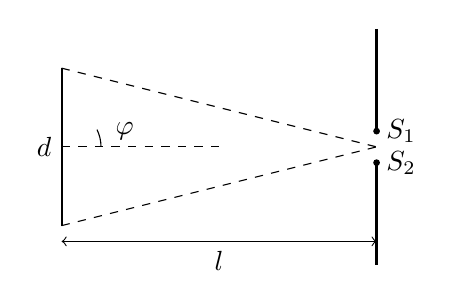
\begin{tikzpicture}
		% Extended source
		\draw[thick] (-2, 1) -- (-2, -1) node[midway, left] {$d$};
		\draw[dashed] (-2, 0) -- (0, 0);
		
		% Slits
		\draw[thick] (2, 1.5) -- (2, 0.2);
		\draw[thick] (2, -0.2) -- (2, -1.5);
		\filldraw (2, 0.2) circle (1pt) node[right] {$S_1$};
		\filldraw (2, -0.2) circle (1pt) node[right] {$S_2$};
		
		% Rays from source edges to center
		\draw[dashed] (-2, 1) -- (2, 0);
		\draw[dashed] (-2, -1) -- (2, 0);
		
		% Angle phi
		\draw (-1.5, 0) arc (0:26:0.5);
		\node at (-1.2, 0.2) {$\varphi$};
		\draw[<->] (-2, -1.2) -- (2, -1.2) node[midway, below] {$l$};
	\end{tikzpicture}
\end{figure}

Условие наблюдения интерференции:
\begin{align*}
	x' &\le \Delta x - \frac{l}{d}\lambda \\
	x'_{\text{max}} &\sim \Delta x, \quad x' \sim l \varphi \\
	l \varphi &< \frac{l}{d}\lambda \implies d < \frac{\lambda}{\varphi} \sim l_{\perp \text{ког}}
\end{align*}
$l_{\perp \text{ког}}$ --- длина пространственной когерентности.

\begin{definition}{Источники пространственно когерентные}{spatial_coherence}
	Два источника, расположение которых позволяет наблюдать интерференцию.
\end{definition}

Объем когерентности: $V_{\text{ког}} = l_{\text{ког}\parallel} \cdot l_{\perp 1} \cdot l_{\perp 2}$.